% Exemple de graphique pgfplots - Puissance THz vs Fréquence
% À inclure dans vos chapitres avec % Exemple de graphique pgfplots - Puissance THz vs Fréquence
% À inclure dans vos chapitres avec % Exemple de graphique pgfplots - Puissance THz vs Fréquence
% À inclure dans vos chapitres avec % Exemple de graphique pgfplots - Puissance THz vs Fréquence
% À inclure dans vos chapitres avec \input{figures/puissance_thz_exemple.tex}

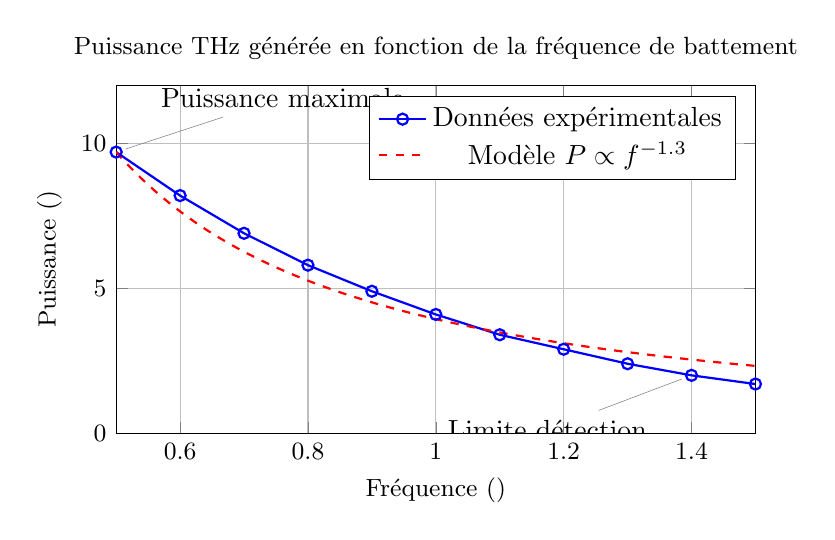
\begin{tikzpicture}
\begin{axis}[
    width=0.8\textwidth,
    height=6cm,
    xlabel={Fréquence (\si{\THz})},
    ylabel={Puissance (\si{\micro\watt})},
    title={Puissance THz générée en fonction de la fréquence de battement},
    grid=major,
    legend pos=north east,
    xmin=0.5, xmax=1.5,
    ymin=0, ymax=12,
    tick label style={font=\small},
    label style={font=\small},
    title style={font=\small}
]

% Données expérimentales (exemple)
\addplot[
    color=blue,
    mark=o,
    mark size=2pt,
    thick
] coordinates {
    (0.5, 9.7)
    (0.6, 8.2)
    (0.7, 6.9)
    (0.8, 5.8)
    (0.9, 4.9)
    (1.0, 4.1)
    (1.1, 3.4)
    (1.2, 2.9)
    (1.3, 2.4)
    (1.4, 2.0)
    (1.5, 1.7)
};

% Modèle théorique (loi de puissance)
\addplot[
    color=red,
    dashed,
    thick,
    domain=0.5:1.5,
    samples=100
] {9.7*(0.5/x)^1.3};

\legend{Données expérimentales, Modèle $P \propto f^{-1.3}$}

% Annotations
\node[pin=45:{Puissance maximale}] at (axis cs:0.5,9.7) {};
\node[pin=225:{Limite détection}] at (axis cs:1.4,2.0) {};

\end{axis}
\end{tikzpicture}

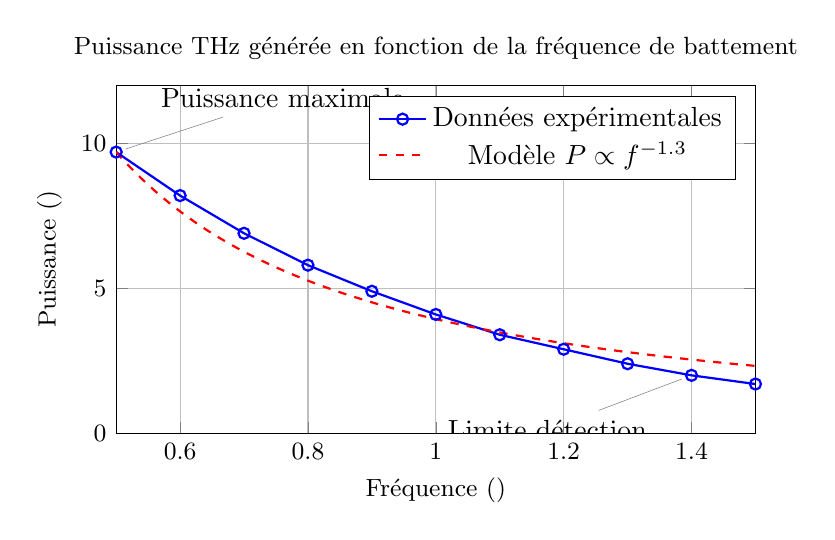
\begin{tikzpicture}
\begin{axis}[
    width=0.8\textwidth,
    height=6cm,
    xlabel={Fréquence (\si{\THz})},
    ylabel={Puissance (\si{\micro\watt})},
    title={Puissance THz générée en fonction de la fréquence de battement},
    grid=major,
    legend pos=north east,
    xmin=0.5, xmax=1.5,
    ymin=0, ymax=12,
    tick label style={font=\small},
    label style={font=\small},
    title style={font=\small}
]

% Données expérimentales (exemple)
\addplot[
    color=blue,
    mark=o,
    mark size=2pt,
    thick
] coordinates {
    (0.5, 9.7)
    (0.6, 8.2)
    (0.7, 6.9)
    (0.8, 5.8)
    (0.9, 4.9)
    (1.0, 4.1)
    (1.1, 3.4)
    (1.2, 2.9)
    (1.3, 2.4)
    (1.4, 2.0)
    (1.5, 1.7)
};

% Modèle théorique (loi de puissance)
\addplot[
    color=red,
    dashed,
    thick,
    domain=0.5:1.5,
    samples=100
] {9.7*(0.5/x)^1.3};

\legend{Données expérimentales, Modèle $P \propto f^{-1.3}$}

% Annotations
\node[pin=45:{Puissance maximale}] at (axis cs:0.5,9.7) {};
\node[pin=225:{Limite détection}] at (axis cs:1.4,2.0) {};

\end{axis}
\end{tikzpicture}

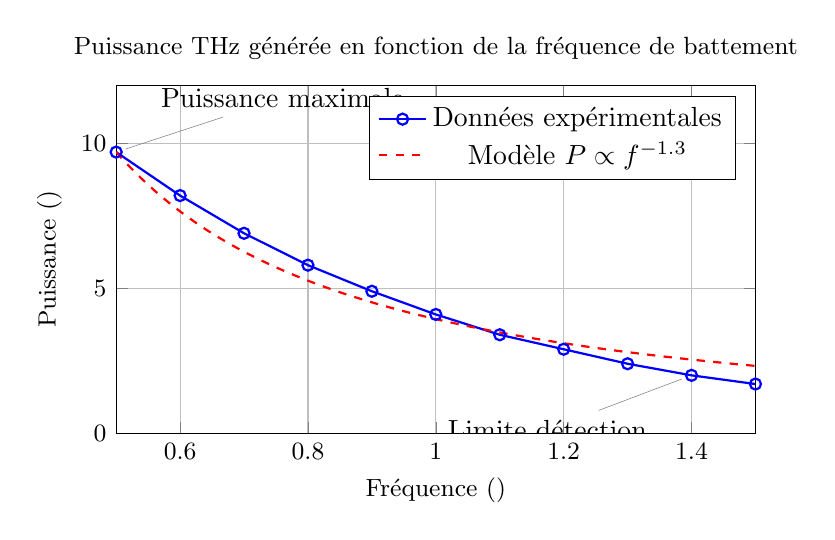
\begin{tikzpicture}
\begin{axis}[
    width=0.8\textwidth,
    height=6cm,
    xlabel={Fréquence (\si{\THz})},
    ylabel={Puissance (\si{\micro\watt})},
    title={Puissance THz générée en fonction de la fréquence de battement},
    grid=major,
    legend pos=north east,
    xmin=0.5, xmax=1.5,
    ymin=0, ymax=12,
    tick label style={font=\small},
    label style={font=\small},
    title style={font=\small}
]

% Données expérimentales (exemple)
\addplot[
    color=blue,
    mark=o,
    mark size=2pt,
    thick
] coordinates {
    (0.5, 9.7)
    (0.6, 8.2)
    (0.7, 6.9)
    (0.8, 5.8)
    (0.9, 4.9)
    (1.0, 4.1)
    (1.1, 3.4)
    (1.2, 2.9)
    (1.3, 2.4)
    (1.4, 2.0)
    (1.5, 1.7)
};

% Modèle théorique (loi de puissance)
\addplot[
    color=red,
    dashed,
    thick,
    domain=0.5:1.5,
    samples=100
] {9.7*(0.5/x)^1.3};

\legend{Données expérimentales, Modèle $P \propto f^{-1.3}$}

% Annotations
\node[pin=45:{Puissance maximale}] at (axis cs:0.5,9.7) {};
\node[pin=225:{Limite détection}] at (axis cs:1.4,2.0) {};

\end{axis}
\end{tikzpicture}

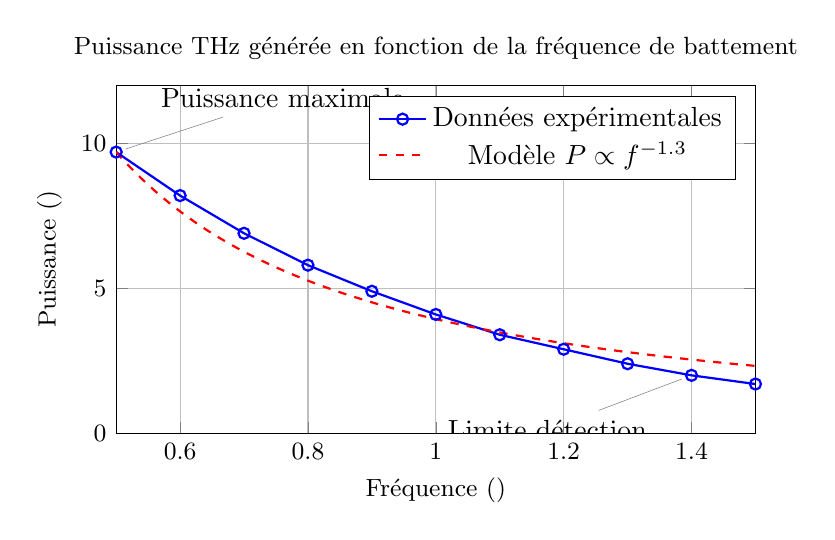
\begin{tikzpicture}
\begin{axis}[
    width=0.8\textwidth,
    height=6cm,
    xlabel={Fréquence (\si{\THz})},
    ylabel={Puissance (\si{\micro\watt})},
    title={Puissance THz générée en fonction de la fréquence de battement},
    grid=major,
    legend pos=north east,
    xmin=0.5, xmax=1.5,
    ymin=0, ymax=12,
    tick label style={font=\small},
    label style={font=\small},
    title style={font=\small}
]

% Données expérimentales (exemple)
\addplot[
    color=blue,
    mark=o,
    mark size=2pt,
    thick
] coordinates {
    (0.5, 9.7)
    (0.6, 8.2)
    (0.7, 6.9)
    (0.8, 5.8)
    (0.9, 4.9)
    (1.0, 4.1)
    (1.1, 3.4)
    (1.2, 2.9)
    (1.3, 2.4)
    (1.4, 2.0)
    (1.5, 1.7)
};

% Modèle théorique (loi de puissance)
\addplot[
    color=red,
    dashed,
    thick,
    domain=0.5:1.5,
    samples=100
] {9.7*(0.5/x)^1.3};

\legend{Données expérimentales, Modèle $P \propto f^{-1.3}$}

% Annotations
\node[pin=45:{Puissance maximale}] at (axis cs:0.5,9.7) {};
\node[pin=225:{Limite détection}] at (axis cs:1.4,2.0) {};

\end{axis}
\end{tikzpicture}